\section{05}

\subsection{05}

primary在节点间分布不均,导致各节点恢复进度差别较大。

每个节点上恢复速度受什么制约?

恢复性能分析:用流体动力学模型。分调度器和下游处理节点。调度能力应大于下游处理能力。
怎么评估main thread的调度能力。

性能分析工具
\begin{enumbox}
\item perf
\end{enumbox}

网络层RPC
\begin{enumbox}
\item 并行
\item libev
\end{enumbox}

磁盘修复不回溯stale数据,为什么?

\subsection{05}

测试发现,从某个epoch起,\hl{scli node recovery总是返回nan},即便停止故障模拟,recovery无法进行。

看standby相关日志,可以很容易发现问题所在,后续收到的只有193的消息,没有收到过192和192的消息,为什么?
进而仔细分析\hl{start recovery和run next rw}两个过程。

run next rw里的cur在某个时间点之后再没有变更过,说明了什么问题?其状态为prepare list,无法推进了。
进一步的分析表明,\hl{该rinfo没有进入recovery的任务队列}。

多次recovery被压缩为两次事件,需要小心管理\hl{recovery的上下文切换}过程。
worker线程用到的rinfo,不允许被main thread free掉。上下文切换的过程,目前的实现也涉及与zk的交互。

不变式:任一rinfo,都需经过free过程。满足malloc/free的对称性。可以用上下文切换的语义建模,辅助理解。

每次recovery周期,update epoch可能被调用一次或两次,视start recovery里新创建的rinfo是否放入next rinfo而定。

\hrulefill

可以用egrep的OR方法,保留多个相关日志的相对顺序,便于分析。如\hl{start\_recovery|free\_recovery\_info|standby|prepare}模式。
欲设计出诊断问题的模式,需要对系统的运行机制有全面而清晰的理解。

发现的问题:
\begin{enumbox}
\item retry逻辑,导致当前恢复周期很长时间才退出,
\item 192异常退出后,191一直恢复失败。
\item 数据跑到stale下面,恢复没有完成,vdi list堵塞。
\item 大量数据被放置在stale下,导致磁盘空间满
\end{enumbox}

移动对象容易带来问题,\hl{需要设计不移动对象的数据管理方案}。
另外,如果采用raw disk方式管理磁盘,如果轻量地移动对象呢?raw disk可是没有rename特性的。

完成队列采用polling机制,不一定要main线程去做?

内部retry逻辑影响到run next rw,进而影响到整个系统的响应能力。
block式网络io也有很大问题。

\hrulefill

\hl{worker thread request done}包括多个完成队列,如rx main、tx main、recovery object main等。
rx main和tx main需要进一步测量其性能,不能是慢操作。

或者是有\hl{多个main线程},去承担节点内所有负载?
切分任务到不同的main线程,任务进行局部化管理。参考lich的core线程设计。

选择什么标准划分任务?任务类型包括:IO、recovery等。

rpc和corerpc的区分:corerpc处理与对象IO,其它请求通过rpc来做?
对象IO可以按照对象hash到不同的main thread上。部分请求是不涉及对象的。

\hrulefill

notify standby发起消息,当master收集到足够的消息后,触发recover peer过程。

\hrulefill

QoS,不限制需要优先恢复的对象。

埋点在工作线程上,故需要线程安全。

\subsection{07}

准备切入全闪方面的工作,ssan的工作大概到五月底。

分布式块存储系统是能力核心,扩大了说就是分布式系统,体系结构方面。
AI是下几年的学习重点。\hl{向Jeff Dean学习},能横跨体系结构和AI多个领域。
合而言之,就是ABC的细分领域。

全面认识ssan的价值,部分c代码和设计是可以重用的。

wd和stale可以理解为COW过程。update epoch是创建对象snapshot的过程。

\subsection{08}

192上的ssan无响应,用\hl{strace/gdb跟踪}了一下,发现陷入sd read lock的循环内。
进一步推测在finish object list里访问rinfo是无效的,被free了。

进一步检查日志发现,rw被生成了两次,一次是init状态,一次是prepare状态。
在执行第二个rw时,关联的rinfo已被freed。

sd read lock的实现,类似于retry逻辑,在某些情况下,会严重影响系统的响应能力。
main thread无限循环,系统永远不再工作。

在update epoch之后,如果无法完成修复,会有大麻烦。

\hrulefill

可追踪性是一项重要的能力,举凡log、stap、gdb、perf,都意味着trace。

egrep分析日志的模式:
\begin{enumbox}
\item start recovery | free recovery info
\item default update epoch
\item ***
\item standby | recover peer
\item queue recovery work
\item prepare | finish object list
\item ***
\end{enumbox}

\hrulefill

改进ssan
\begin{enumbox}
\item 大量LOG
\item 引入GOTO、assert
\item 产生coredump
\item check and set rlimit
\item 双进程结构
\item 可扩展的main线程
\item 调整epoch目录结构
\item 并发网络请求
\item rinfo状态机,并发下的引用计数
\end{enumbox}

\hrulefill

战略要义在于一。\hl{舍九取一,取一是主要方面}。有所为有所不为,有所为是主要方面。

没有记录的公司是没有希望的,同样,没有记录的个人成长也值得怀疑。
一旦确立长期观点,就可以深谋远虑,变得从容主动。

一是综合判断,聚焦,不排斥多元的变化,蕴涵无尽可能。

道生一,无极而太极。一即是战略,又是战术。后面的数字偏于分析。

吾道一以贯之。天下之道,可一言而尽也:其为物不二,则其生物不测。

少年得志可喜,大器晚成可贵。有目标,沉住气,踏实干。

天下之动,贞夫一者也。找到人生的这个一,即是使命。

老子传奇里,某位真人对老子的教导,就强调了这个一字。阳明归纳而又归纳,得出致良知一法门。
孔子曰:吾道一以贯之。商君一言,利出一孔、利出一孔,处处显出一的可贵。有个这个一,则万象生。
爰有奇器,是生万象。

\hrulefill

update epoch是非常危险的操作,且耗时,且由main thread来完成,故必须优化。

\subsection{09}

ssan测试出来的问题
\begin{enumbox}
\item update epoch耗时极多,堵塞main thread
\item 加入节点时,do get vdis发生panic,原因是其它节点在进行耗时的update epoch
\item stale object GC
\item disk full,恢复无法继续,会丢数据
\end{enumbox}

\hl{重新format集群时,需先行卸载各个卷}。否则,貌似有问题。

rinfo状态机
\begin{enumbox}
\item 何时放入工作队列
\item oid in recovery
\item 能否取消,开始下一周期
\end{enumbox}

\hrulefill

性能之巅一书,结构很是合理。\hl{文件系统和数据库系统},复杂度很高。

ssan的精髓是什么?

需要有自己的作品和名片。

\subsection{10}

用epoch管理数据和处理逻辑,epoch是一个全局大版本。版本在分布式系统里有着广泛的应用。
但epoch粒度过大,有些逻辑难以处理。看待问题有两个角度:版本和对象。对象随着版本在演化。

notify standby如果收集不到足够的消息,就会堵塞整个修复进程。
此时如果有新的修复事件,应该可以取而代之,把恢复过程推向前进。

回收stale object,需要独立的GC过程。\hl{GC与IO、Recovery}各个过程之间需要一定的同步机制。

通过策略模式提炼并行send reqs。适配和策略。

vdi check没有检查vdi对象,目前ssan的副本修复机制感觉有问题,\hl{选择何者为权威}是一个没有得到证明的过程。

用valgrind分析内存问题很给力。

与epoch相关问题
\begin{enumbox}
\item rebuild stale list too long
\item 对象在文件系统上如何组织,包括wd和stale的区分
\item recovery过程占用空间与数据量的关系,空间利用率有多高
\item 恢复中的GC策略和独立的GC过程
\item ***
\item 木桶原理
\end{enumbox}

\hrulefill

\begin{enumbox}
\item 为什么要移入stale目录?
\item rename是否必要
\item epoch不变的情况如何处理
\item GC策略是什么?回溯至最高可用版本?
\end{enumbox}

rebuild stale list只在磁盘故障时有必要,移除故障盘上的相关记录。
单纯节点修复时,本节点stale list无变化。

stale list本质上是对象在各个磁盘上的存储结构。
每个对象可包含如下属性:\hl{oid、epoch、idx、diskid、version}等。

object list cache可由stale list推导而来,即是stale list的keys。
stale list的相关信息,只对EC卷有用。副本卷只需要object list的信息。

\hl{GC过程}需要stale list,本节点的stale list信息并不够,
对任一对象而言,还需看别的节点的相关信息。

结论:object list cache作为对象在磁盘上的分布的一种反映。
提供接口给上层应用使用,如get tgt epoch,get object list。

\subsection{14}

统一stale list cache和object list cache,处理好CRUD等操作
\begin{enumbox}
\item load
\item create and write | link
\item remove object
\item remove stale versions
\item move from wd to stale
\item change diskid
\end{enumbox}

某一数据分片<oid, idx>在某节点上有一个或多个版本<epoch>,存放在特定的disk上<diskid, wd>。
多个版本构成版本历史,用动态数组管理,按epoch降序排列。

跟踪大型数据结构的内存占用量。

\hrulefill

集中心力思考大事要事,切己体察,多讲利益,少讲价值观。

\subsection{15}

刊落声华,一意本源。

有目标、沉住气、踏实干。

验证stale cache与底层对象分布的一致性。

为什么get tgt epoch返回空结果,后续如何处理?

stale cache按epoch组织,是否有一个epoch对应多个数据分片呢?
wd和stale什么情况下具有相同的epoch?如何处理?

vdi object特别处理,其epoch和index规则均不同。

等待的时候可以写日志。中年焦虑,反正下一帐必须赢,浪费不起了。
一寸光阴一寸金,寸金难买寸光阴。

\subsection{16}

观察分析恢复的空间复杂度。算法要从多个指标上去评估,主要是时间和空间复杂度。

加强断言,能发现一些隐藏的bug。

维护磁盘上对象结构的内存映射比想象中的要复杂。要始终一致。
如果出现不一致,可以增加重新加载的机制。
\begin{enumbox}
\item 如update epoch失败会如何?get tgt epoch返回错误结果。所以,\hl{务必要确保update epoch能正常完成}。
\item \hl{create and write跨start recovery},都成功了,导致wd下有两个版本的对象,epoch不同。
\item link与create and write同,也产生了新对象。
\item \hl{优先加载vdi},很多操作依赖于vdi state信息。
\item 191退出,fio不退出,mount3一直无法完成。
\end{enumbox}

\subsection{17}

需要密切注意的是,add和remove在各种粒度上的对称性,粒度包括:对象,对象之epoch等。
不同层次或粒度都是物质不灭、能量守恒的。物质不灭或不为真,能量守恒则必为真。

今天是在东升科技园的最后一天,搬家去技术转移中心。外界之境遇在变,我心不变。
\hl{存在是一},巴门尼德的这个认识极有深度。一是系统观,二是本体论。

\hl{郝拉克里特}说得是现象界的流变及其动力,巴门尼德说的是本体界、物自体。

object list cache通过version来跟踪变化情况。

stale cache的数据项,按\hl{oid, epoch, index, diskid, wd}进行区分。缺少一项就有可能出问题。
<oid, index>代表数据分片,<diskid, wd>代表物理位置,epoch代表版本。注意副本和EC的同和异。

stale cache转化为磁盘上对象分布的cache,包括\hl{wd和stale对象}。在此之上,导出相关API。

\hrulefill

回到原点,所以需要恢复,就是因为对象的缺失或错位。
节点故障和磁盘故障都可以导致缺失或错位。

数据不一致现象呢?如何检测?基于内容的hash、或version机制。

对有元数据的系统,则无错位的现象。

\hrulefill

延展集群

心无旁骛,专注于一事。

\subsection{20}

战略,大处着眼、小处着手的大处。无战略,悲人生。
盲目地做事情,就有赖于机遇。

战略研究四境界:历史、科学、艺术、哲学。很精辟。
S是战略、是成功,战略是制胜之道,没有战略何谈成功呢?
同时,S也是太极的S曲线,曲则全,曲成万物而不遗。

秉承黄老传统,两大命题:\hl{道生一,道生法}。前者入哲学之域,后者入战略之门。

战略之追求在于行动自由,致人而不致于人。何以致之?修道而保法,故能为胜败之政。

产品是战略的物质载体,不可谓不重也。

\hrulefill

指标分时间和容量两方面。io中断时长、降级下的性能是时间方面的指标,
额外的空间占用是容量方面的指标。与算法分析类似,\hl{时间复杂度和空间复杂度}。

\subsection{21}

阳光照耀大地,通天接地,双线法则。天之命题:道生一,地之命题:道生法。
哲学、战略之同异犹如天地。\hl{哲学、战略、战术}如连环。常山之蛇。

\hl{大处着眼、小处着手}。基础和前沿,两者要兼顾。

晚上的时间,不用太忙于工作,复盘、刻意练习,打基础,跟踪前沿。
日积月累,持之以恒。

\hrulefill

unlink stale object看上去也不是并发问题,是什么导致cache和磁盘上结构不一致呢?
unlink为什么返回ENOENT,在哪里删除了呢?

可以通过两个计数器来判断是否出现了并发。

ssan上不再实现新功能,一是bugfix,二是设计。
\begin{enumbox}
\item 副本一致性机制
\item 性能
\item 异步通信
\end{enumbox}

\hrulefill

DHT的不足之处,一旦ring任一节点发生变化,\hl{实际问题与计算位置}就不一致。
需要尽快纠正,因为EC要求严格顺序,情况会更复杂些。

\hl{thread pool and work queue},好好体会一下。一个线程池处理一个提交队列,一个完成队列。
完成队列可以与别的线程池共享。\hl{线程池中的每个线程,处理提交队列的任务,完成后,加入完成队列}。
由polling thread处理完成队列。

任务都嵌入了work对象,指定所需的callback函数。

\subsection{22}

分布式系统,先看\hl{数据模型、协议、算法}等。
\hl{通过wiki或其它途径进行scan},官网可以了解有什么,然后多方途径,探知其why and how。

\begin{enumbox}
\item 华为
\item BAT
\item TMD
\item 浪潮
\end{enumbox}

博采众长,研究几个系统:
\begin{enumbox}
\item FusionStor
\item SheepDog
\item Ceph
\item *** File and Object
\item GlusterFS
\item Qumulo
\item Isilon (DELL/EMC)
\item Lustre
\item *** DB
\item sqlite3
\item Redis
\item MongoDB
\item LevelDB/RocksDB
\item Pegasus (XiaoMi)
\item TiDB
\item OceanBase
\item ***
\item SPDK/DPDK
\item QEMU
\end{enumbox}

Ceph的PG概念,一个pool内PG数目相对固定,调整PG数目会引发大量数据迁移。
PG有几个特点:object映射到PG,PG映射到OSD,第二层映射与副本和EC有关,
所以副本和EC都是按pool指定的。\hl{如果PG数目不变,则第一层映射不变}。

Redis的hash slot又是如何解决这个问题的呢?

视野要放到数据存储和管理行业,包括公司、人物、技术前沿。

\hrulefill

Redis的数据模型,基本数据模型是KV,V可以是一个数据结构。

\hrulefill

c语言中\hl{array和struct的初始化语法}类似,分别采用索引或成员表达式指定对应的成员,不指定的采用默认值。

EC中特定情况下需要log,如果按读改写逻辑,记录整个条带到日志,就不需要UNDO日志,用单一的REDO日志即可。
RAID5就是这么做的(张东)。

pool、vol、snapshot数据在etcd上保存,vol的元数据采用MDS。

IO路径由client直达数据存储端,不经过控制器中转了。支持多个client端访问一个数据,
有subvol controller负责同步,具体地说就是每次io需要申请一个token/version,
IO按object version语义规则进行。

读改写发生在client上,数据存储端收到的都是对齐的条带。

EC所需LOG不必引入LOG volume,而是放在数据分片的物理层上。
采用两阶段提交协议,来实现原子写。

\subsection{23}

战略,取舍,战而胜之。兵道接近生活之真义,在竞争中战而胜之,得行动自由。

孙子更言兵道之重要,国之大事,死生之地,存亡之道,不可不察也。
如何察之?道天地将法,孙子尚五。

\hrulefill

新发现的问题:

update epoch后,有create and write,后面才有prepare object list,导致对象无法恢复。
create and write不被block,节点恢复又是基于stale数据。

master recover peer work如果遇到不可用sockfd,需要重试。否则,无法唤醒部分节点,
导致部分节点恢复正常进行,部分节点不能进入prepare阶段。总的结果是恢复无法进行。

与一个节点sockfd cache有多个fd,如果retry仍然失败呢?

观察master recover peer的重试次数。

每个节点finish object list时机不同,所以每个节点上\hl{恢复开始有先有后}。

standby过程不可少,需要完成object list cache的构建,后续prepare object list的结果才是正确的。

\subsection{24}

世界虽大,忘战则小。小到没有生存空间,丧失行动自由。
此多年切实之体会,回到兵道。\hl{我欲清溪寻鬼谷,不论礼乐但论兵}。
诗和远方需要强大的后备力量支撑,空口白话无意义。

没有斗争意识,奋斗精神,世界的宝藏不会向你开放的。

兵道并非蛮力,乃是一生存权的竞争,东方兵道具有哲学和战略的高度。

\hrulefill

磁盘空间利用率过高时,如需要恢复,可能无法完成。如何解决该问题?

在finish object list进行检查,需要具体到每个磁盘是否有可用空间,同时还需跟踪记录create and write的占用情况。
磁盘空间由三部分占用:wd、stale,还有新生成的。

如果空间不足,则标记当前集群状态,并退出该次修复。按集群状态处理各种操作。
如可以删除卷以回收空间,回收空间后,重新检查。

与shutdown的处理方式有类似之处。shutdown是单向不可逆的过程,标记空间不足则是可逆过程。

\hrulefill

怎么确保move to stale过程总是成功的呢?

按epoch组织目录结构,就不需要移动object了。\hl{因为磁盘故障不提升epoch,则需特别处理}。

\hrulefill

文以载道,要超级重视写作了,不能再乱打仗,言有宗,事有君。

\subsection{27}

本周任务:
\begin{enumbox}
\item 填写转正申请表
\item 完成ssan交接文档
\item 开始全闪方面的PDCA循环/规划工作
\item ***
\item 周末填写积分落户申请
\end{enumbox}

\subsection{28}

转到全闪方向,需要补充哪些知识?
\begin{enumbox}
\item 存储和网络
\item SPDK/DPDK
\item 多点写入?
\item snapshot and consistency group
\item ***
\item Docker
\end{enumbox}

采用小步快跑的开发模型,稳扎稳打、步步为营。
第一阶段,完成一个MVP,最小可行产品。然后在此基础上滚雪球。

需要验证的指标,集中在一致性和性能两方面,\hl{用功能对架构进行压力测试/思想实验}。
搭建测试框架,实践TDD最佳实践。

从\hl{架构、产品、项目}几个维度进行综合考量。A级架构师的架构、战略、商业都是相关的。
\hl{架构在战略和商业之间的桥梁作用}。

控制一下范围,\hl{设计内置质量},特别是测试框架,放到非常重要的位置。

\hrulefill

周一例会之前发周报。

项目的质量三角:范围、成本、时间。
\begin{center}
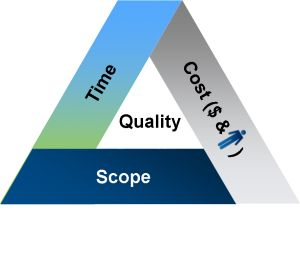
\includegraphics[width=8cm]{../imgs/quality.jpeg}
\end{center}

\hrulefill

持久化数据:
\begin{enumbox}
\item etcd
\item bactl上的persistence array和chunk
\end{enumbox}

persistence array是卷的二级元数据。

\hrulefill

介玄克讲glusterfs的元数据,通过fuse导出的分布式文件系统。主要问题是什么?小文件、ls效率。
当存在海量文件时,ls效率极差。如何解决?解决方案分两类:局部优化、全局优化。

dir readahead 没有管理好cache,一直在累积,没有释放,导致内存使用量过大。

全局优化也分两类:缓存、元数据中心。

glusterfs的translator是个良好的抽象?很多特性都是以translator的形式存在?

对标别的系统:
\begin{enumbox}
\item 爱奇艺用的是glusterfs?不是换成open vstorage了吗?
\item ceph的文件系统也是引入了文件系统元数据,似乎处理的并不好。
\item 在目录级别设置副本、或EC策略
\item minio的设计亮点?
\end{enumbox}

\hrulefill

从经历中学习,全情投入模型:方法、行动、反思。哪些经历发生了重要的影响呢?
简历上通常有学习经历和工作经历。应该还有其它的方面。

聚焦到培养能力上,特别是专业能力,很多经历没有得到很好的反思,没有转化为相应的能力。
就近而言,入职大道以来的那么多经历,哪些是得到认真反思和回顾的?又提升了哪些能力?
要时刻保持在学习的状态,“三人行必有我师焉”,谦受益、满招损。

比如演讲,一直回避,不去面对,问题始终得不到解决。
演讲和说服是很重要的能力,为什么避而不谈,不去积极解决呢?

\subsection{29}

反思影响圈和关注圈的分别,印象深刻。最近关注圈太大,影响圈反有所不及,当及时调整。
最内层再加一个能力圈的概念,就是巴菲特一直强调的护城河。

在强调能力圈和影响圈的同时,并非不要关注圈。科技前沿要关注,在交叉地带去开拓,说不定能带来惊喜。
这种内外之别,中庸有特别好的表达。合内外之道,故时措之宜也。\hl{致广大而尽精微,极高明而道中庸}。

当前之抓手何在?全闪架构+AI,沿着这个赛道,前途一片光明。要有这个确信,可以集中一切力量,

如何理解\hl{价值投资}?选择好赛道,长期持有。择善固执是通往从容中道的阶梯。

同心圆模型:\hl{孙老二子},也构成同心圆,内圣外王。

\hrulefill

阿里多隆,扫地僧,一股傻劲,任正非提及的阿甘,都是\hl{傻人有傻福}。
\hl{切勿三心二意,务必全情投入}。

\hl{经历驱动的领导力开发},这个意味好。复盘的指向性不够,领导力开发是复盘的目的之一。

\subsection{30}

\hl{沙克尔顿的领导艺术}中提炼了十大原则,近期要记下来好好消化。奈飞文化手册也有同等价值。
重要的不是牢记条文,而是领悟其实质,化为切实的行动计划。

\hl{第一条:牢记最终目标,集中力量实现短期目标}。探险之旅是一个隐喻,最终目的地是哪儿?
我是谁?从哪里来?到哪里去?这里所谓的哲学三问。

四十五岁前能实现财务自由吗?还有三年时间,很有挑战,但并非不可达。
目标一定要足够大,还能激发斗志,全情投入。

不积跬步无以至千里,最终目标是一步一步达成的,
中间设定里程碑,小步快跑,稳步推进。

\hl{第四条:保重自己}。特别重要,要有自我调节之法,
保养精气神。参考鬼谷子阴符七篇,盛神居于首位,依次有\hl{盛神、养志、实意、分威、散势、转圜、损兑}。
涉及心性、思维、战略等方法面面。静和者养气,养气得其和。

\hl{Be endurance we conquer}。坚毅者胜。坚毅不是无指向的,
而是在追求使命的过程中,表现出的必要特质。

\hrulefill

任正非读书法:
\begin{center}
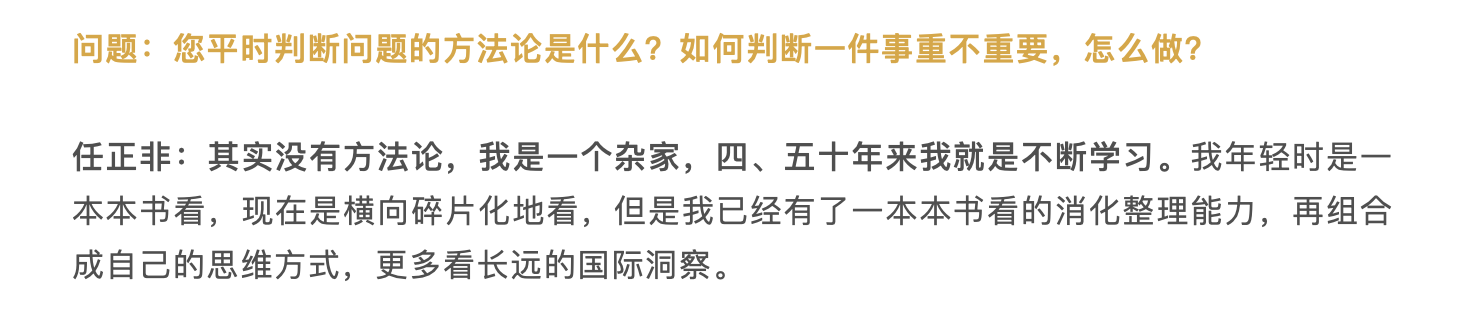
\includegraphics[width=11cm]{../imgs/renzhengfei-reading.png}
\end{center}

下面是一个倒V,上面是一个V,合起来就是X。bottom up的顶天立地。
形成X的中间一点是至关重要的一步。

\hl{从厚到薄,从薄到厚},中间的焦点,就在于形成自己的思维方式和整合能力,
亦是\hl{铁棒磨成绣花针}。其针尖战略,发人深省。

任自认为杂家,杂中取其一点。\hl{读万卷书、行万里路、做一件事}。
万和一之间相辅相成。

\hrulefill

沉静下来,做持久战,没必要太沉不住气,一切都是最好的选择,纵情向前。

要做战略思考,反思过往,曲折甚多,不能达于本源。

分布式存储从纵深看,也是一大产业,与云、大数据、AI都密切相关。

\subsection{31}

pingcap值得追踪一下。
